\chapter{Background\label{cha:background}}

The 2010 Formula SAE vehicle is essentially made up of five functional systems, namely the \emph{engine}, \emph{transmission}, \emph{braking}, \emph{telemetry}, and \emph{driver interface} systems. The background of these systems is discussed further in this chapter, to provide the reader with the knowledge required to follow the reasoning for our design. The specific vehicle components that interface with the four electronic modules and the electro-pneumatic system are annotated in Fig. \ref{fig:background_overview_topdown}. 

\vspace{1em}
\begin{figure}[H]
\centering
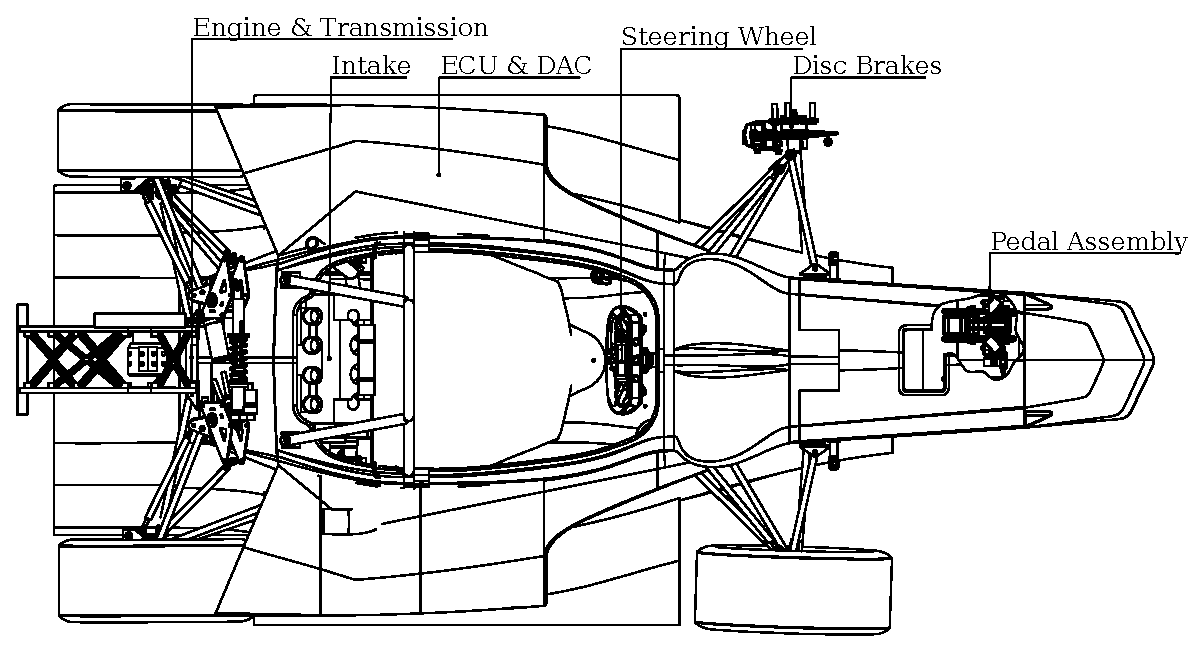
\includegraphics[width=6in,keepaspectratio]{background/figures/background_diagram.eps}
\caption{Top-down view of the 2010 Formula SAE vehicle.}
\label{fig:background_overview_topdown}
\end{figure}

\section{Engine}

\subsection{Overview}

brief {}``what is engine'', honda cbr, etc.

maximise power output (performance application)

torque power curve, etc.

\subsection{ECU}

A specialized third-party component called the \emph{Engine Control Unit} (ECU) controls the fuel injector and spark coil systems that in turn control the combustion cycle of the engine. The particular model of ECU used by the Formula SAE car is the S80Pro from DTAFast \cite{s80pro}. The ECU uses the O$_{2}$, MAP, cam position, and crank position sensors to adjust the fuel injector and spark coil timings. This keeps the engine running smoothly. The ECU features a traction control system that monitors wheel slip and cuts spark and fuel to provide traction when one of the wheels is slipping. The ECU also collects the various sensor readings and makes them available to other electronic devices at a fixed frequency through a shared data bus. 

\begin{figure}[H]
\centering
%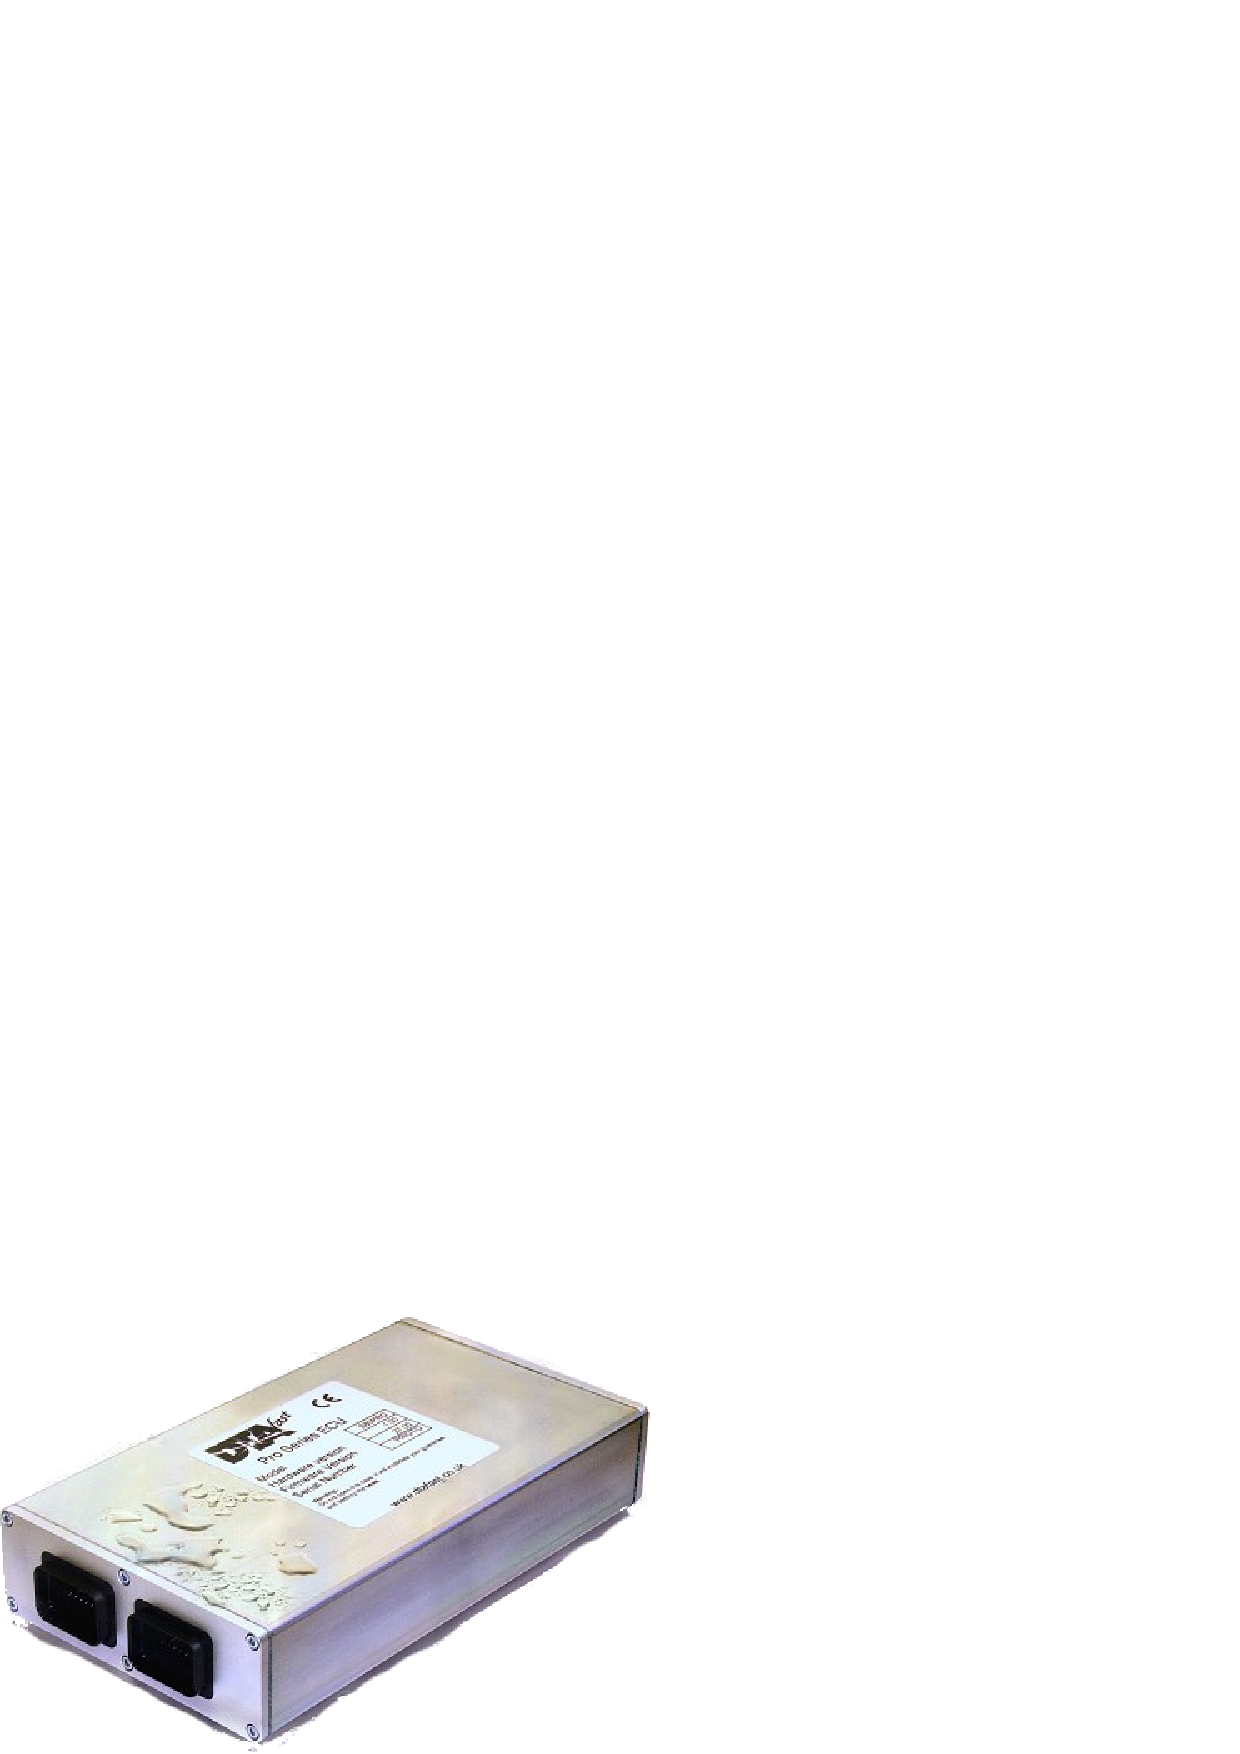
\includegraphics[scale=0.5]{Figures/s80.png}
\caption{The DTAFast S80Pro engine control unit.}
\label{fig:s80pro_product}
\end{figure}

\subsubsection{ECU Data interfaces\label{sec:background_ecu_data_interfaces}}

The ECU provides 3 digital communication methods:
\begin{itemize}
  \item An RS-232 link is used by the software that DTA provides for tuning and controlling the ECU. The serial protocol that the software uses is proprietary and undocumented.
  \item A read-only CAN bus interface that emits ECU data at a fixed frequency. The message format for the CAN data is documented in Appendix \ref{cha:ecu_can_spec}.
  \item Several CMOS-level discrete inputs:
  \begin{itemize}
    \item Launch Control toggle, which toggles the launch control feature in the ECU,
    \item Shift cut, which signals the ECU to reduce engine power before a downshift
    \item Traction control toggle, which toggles the traction control feature in the ECU,
    \item Traction control wet/dry, which switches between two different sets of traction control parameters in the ECU.
  \end{itemize}
\end{itemize}

Detailed descriptions of the ECU's launch control, shift cut, and traction control features can be found in the manual \cite{s80pro}.
 
\nomenclature{RS-232}{Recommended Standard 232, a byte-oriented serial communications protocol, typically asynchronous.}

\subsection{Intake and Exhaust}

Intake background, pressure waves, etc. Torque curve depends on length, 

\subsection{Research and Modelling of Variable Length Intake}

present research done by others on team, quantified runner length
dependence

intake length changes power

quantified length versus power on actual vehicle

chose optimal intake length

proposed variable length intake system for future work

\subsection{Starting System}

current requirements, starter motor, etc.


\section{Transmission\label{sec:background_transmission}}

\subsection{Overview}

The Formula SAE 2010 vehicle uses a 6-speed manual sequential transmission to transmit power from the engine to the drive train. As in other types of manual transmissions, the sequential transmission works by engaging and disengaging several sets of gears with shift forks to obtain different gear ratios. A cast steel drum inside the transmission, called the \emph{shift drum}, has a series of complex grooves machined into it, in which the shift forks ride. Rotating the drum causes the forks to engage one gear and disengage the other. A ratcheting mechanism allows a single external lever, called the \emph{shift lever}, to rotate the drum forward and back by a discrete amount. Each full movement of the lever forwards or backwards causes a gear change up or down, respectively \cite{HowtoManualTransmission, cbr600}.

\subsection{Neutral Sensing}

The stock CBR600f4i engine is fitted with a simple 1-wire sensor which is connected to ground when the transmission is in neutral. The wire is left floating when the vehicle is in gear.

\subsection{Gear Position Sensing}

The stock transmission has no means of determining what gear the transmission is in; it can only determine when the transmission is in neutral using the aforementioned neutral sense wire. The ECU has provisions for reading a gear position potentiometer that can be attached to the shift drum, however this requires mechanical modification of the shift drum itself.

\subsection{Clutch}

The CBR600f4i is equipped with a multi-plate clutch which serves to transmit torque from the engine to the drivetrain. Layers of friction plates in the clutch are forced to rotate together when the clutch is engaged by a series of pre-tensioned springs. When the clutch is disengaged externally via the \emph{clutch lever}, the plates are separated and the drivetrain is allowed to spin freely from the engine. The clutch lever is actuated on the stock motorcycle with a hand lever via cable.

\subsection{Starting and Changing Gears}

In normal operation of the car, the clutch is used to accelerate the car from a stand-still, and to down-shift the transmission. Use of the clutch is not required for up-shifting, only a small reduction in engine torque.

When accelerating the car from a stand-still, two sub-cases need to be considered: accelerating at the beginning of a race, which is known as \emph{launching}, and moving the car forward in a slow, controlled, manner, which is known as \emph{crawling}. In launching the car, the goal is to gain as much momentum as possible by transmitting as much torque from the engine to the wheels as possible without causing the wheels to slip. The goal of crawling the car is to accelerate slowly to a speed less than \unit{25}{\kilo\metre\per\hour}.

Manual clutch control requires a significant amount of skill on behalf of the driver. To launch the car with minimal tire slip, the driver must modulate the throttle as well as the clutch. Crawling a Formula SAE car is a similar operation, however it is very easy to stall the engine by engaging the clutch too quickly. It is often desirable to move the car slower than would be obtained by driving in first gear with the clutch fully engaged. To achieve this, the clutch state is alternated between slipping and fully disengaged.

Down-shifting the transmission requires that the clutch be fully disengaged. In a purely manual system, the driver must disengage the clutch, shift the transmission, "blip" the throttle\footnote{``Blipping'' the throttle is a short increase in throttle used to increase the engine RPM in order to match it closer to the clutch plate RPM}, and then re-engage the clutch. This is required since the torque transmitted by the clutch (Eq. \ref{eq:clutch_slip}) can be in the reverse direction, from the wheels to the engine.

\subsection{Previous Electro-pneumatic Implementation}

There are several disadvantages to a purely manual transmission:

\begin{itemize}

\item It requires a great deal of dexterity and effort on behalf of the driver;

\item Shift time is relatively slow (around \unit{1}{\second}) compared to an estimated theoretical minimum shift time ($<\unit{100}{\milli\second}$); and 

\item A mechanical linkage must be designed and packaged into the car.

\end{itemize}

For these reasons, the Formula SAE team replaced the mechanically-actuated system with an electro-pneumatic one in 2007. This new implementation replaced a purely mechanical clutch pedal and gear shifter with pneumatic actuators linked directly to the clutch and gear selector levers. Driver control was achieved with a set of electronic paddle switches located on the steering wheel: an up-shift paddle and a down-shift paddle. A compressed air cylinder is used to feed air to linear pneumatic cylinders, which apply force to the clutch and shift levers. Binary 3-way solenoid valves apply pressure to either side of the cylinders.

The initial control of the solenoid valves was accomplished with a set of switches on the steering wheel. These switched the low-current side of a set of relays, which in turn fed current to the solenoid valves. Actuation of the clutch was entirely dependent on how long the driver held down the paddles. This reduced the required effort from the driver, but still often resulted in missed shifts. It also caused heavy mechanical stress on the transmission as the actuators pressed hard on the shift levers.

The 2008/2009 Formula SAE car improved on the 2007 design by replacing the relays with high-current solid state drivers. The timing signals to the solenoid valves were precisely controlled with an ARM7 micro-controller. Shift timing could be programmed, and no longer depended on how long the paddles were held. This reduced the effort required from the driver and also reduced possible driver error. Although an improvement from previous years, the system is wasteful of air, and the air cylinder must be regularly refilled.

The most serious drawback of either system is that the position of the clutch actuator is binary. It is only possible to engage or disengage the clutch at a constant rate, determined by the pressure in the system, the flow rate coefficient through the valves, and the diameter of the cylinder. Launching the car requires careful modulation of the clutch position, which is not possible with a binary pneumatic system. Thus, launching the car requires a hand-lever.

Another limitation is posed by the lack of gear position sensing in the stock transmission. Although the system is able to determine when the transmission is in neutral, there is no way to determine if the gears have meshed after up- or down-shifting, and the signals sent to the actuator are therefore controlled in an open-loop fashion with static timing tables.

\section{Braking}

The braking system on the 2010 Formula vehicle is a hydraulically-controlled \emph{disc brake} system. Hydraulic pressure causes callipers on each wheel to squeeze friction pads against the discs, thus braking the vehicle. There are two entirely independent closed hydraulic systems, one for the front brakes and the other for the rear brakes. If one of the systems fails, the other system may be used to safely stop the vehicle. 

The \emph{brake pedal assembly} houses the components used by the driver to engage the brakes, including the \emph{brake pedal}, \emph{brake master cylinders}, and an adjustable \emph{balance bar} for changing the front-rear force distribution. Adjusting the force distribution is called \emph{brake biasing}, and can play a dramatic role in the performance of the vehicle. However, proper brake biasing is a tedious and difficult procedure.

\subsection{Brake Pedal Assembly}

A brake pedal in the cockpit is used to engage the brakes. Two \emph{brake master cylinders} (one for the front system and the other for the rear system) are connected to the brake pedal by way of an adjustable \emph{balance bar}. The balance bar distributes force from the brake pedal to the master cylinders \cite{TiltonBrakeBias}. 

The brake pedal, master cylinders, and balance bar are attached to a modular frame that is located at the end of the cockpit. Together, these components form the \emph{brake pedal assembly}. A model of this assembly is shown in Figs. \ref{fig:brake_pedal_assy_a} and \ref{fig:brake_pedal_assy_b}. Removal of the brake pedal assembly is prohibited because the brake lines that connect to the master cylinder cannot be removed without depressurizing both the front and rear brake systems. 

\begin{figure}[h!]
	\centering
		\subfigure[Front view]{
			\label{fig:brake_pedal_assy_a}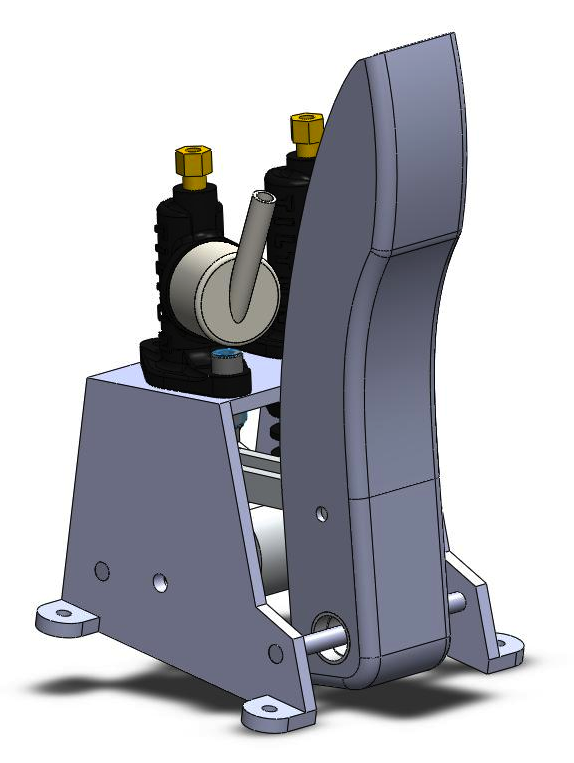
\includegraphics[scale=0.4]{background/figures/brake_pedal_assy_a.eps}}
		\subfigure[Rear view]{
			\label{fig:brake_pedal_assy_b}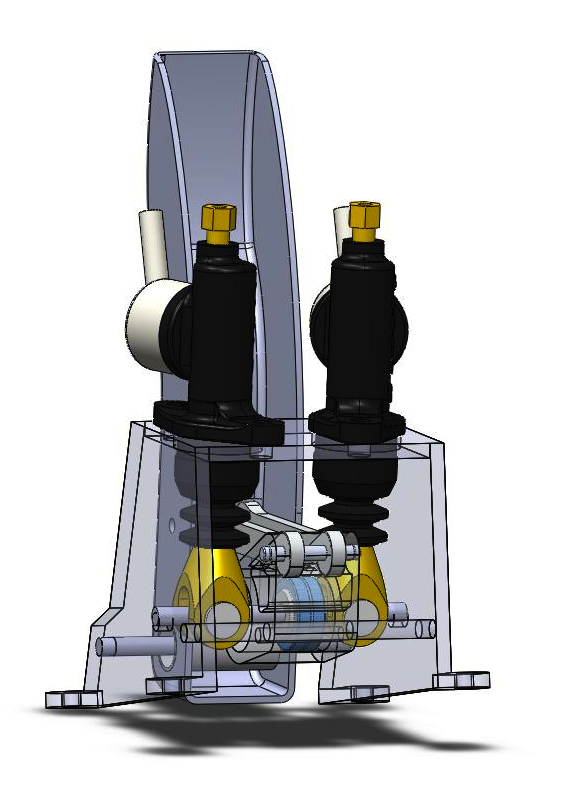
\includegraphics[scale=0.4]{background/figures/brake_pedal_assy_b.eps}}
    \caption{The brake pedal assembly.}
    \label{fig:brake_pedal_assy}
\end{figure}

\subsection{Brake Biasing}

Changing the relative braking force between the front and rear is called \emph{brake biasing}. For example, having 65\% of the braking force applied to the front wheels and 35\% to the rear is denoted as "65/35" brake biasing. 

Most of the vehicle weight is in the rear, where the engine is mounted. During braking, weight is effectively transferred from the rear of the vehicle to the front. This weight transfer reduces the braking force available to the rear tires. If too much rear brake force is applied, the rear tires may lock-up and the vehicle will lose traction \cite{FundVehicleDynamics}. This situation can be avoided by properly biasing the brakes for driving conditions.

The relative force provided to each brake master cylinder can be changed by rotating the \emph{balance bar}. When the balance bar is centred between the front and rear cylinders, an equal amount of force will be applied to each. The relationship between the deviation of the adjusting shaft from it's centre position and the relative force applied to each cylinder is approximately linear for a range between 70/30 and 30/70 \cite{TiltonBrakeBias}. 

\subsection{Difficulties in Bias Adjustment}

Adjusting the brake bias in virtually all previous generations required removing body panels or the front nose cone, and manually turning a knob on the bias bar. Finding an appropriate setting for brake bias was a tedious trial and error exercise, as drivers had to run a lap in the car, brake heavily, and then return to the team so that the body could be removed and the bias adjusted. Often, drivers were unsatisfied with the bias chosen by another driver, which meant a (likely sub-optimal) compromise in bias point had to be chosen.

\section{Telemetry}

\subsection{Overview}

The manufacturers of both the ECU and the DAC provide specialized PC software that communicates with the modules using the serial data interfaces described above. The intended procedure for using these interfaces is by physically connecting a hard serial cable from the modules to a PC running the software. This however limits mobility, and requires the plugging and unplugging of cables.

Why is telemetry necessary? Sensors, data, etc.

\subsection{DAC}

Another specialized third-party component called the \emph{Data Acquisition Device} (DAC) is used to log and relay sensor data to other electronic devices.

The particular DAC used is the model DL1 from Race Technology \cite{DL1Dsheet}. The DL1 is an expandable data logger with built-in \unit{20}{\hertz} GPS and 3-axis accelerometer.

\subsubsection{DAC Data Interface\label{sec:background_dac_data_interface}}

Race Technology provides a software suite that communicates with the DAC using a documented serial protocol. Every item that the DAC logs is output to its own channel in real time on the serial port. It is also possible to configure the software to recognize new channels for arbitrary types of data.

\begin{figure}[H]
\centering
%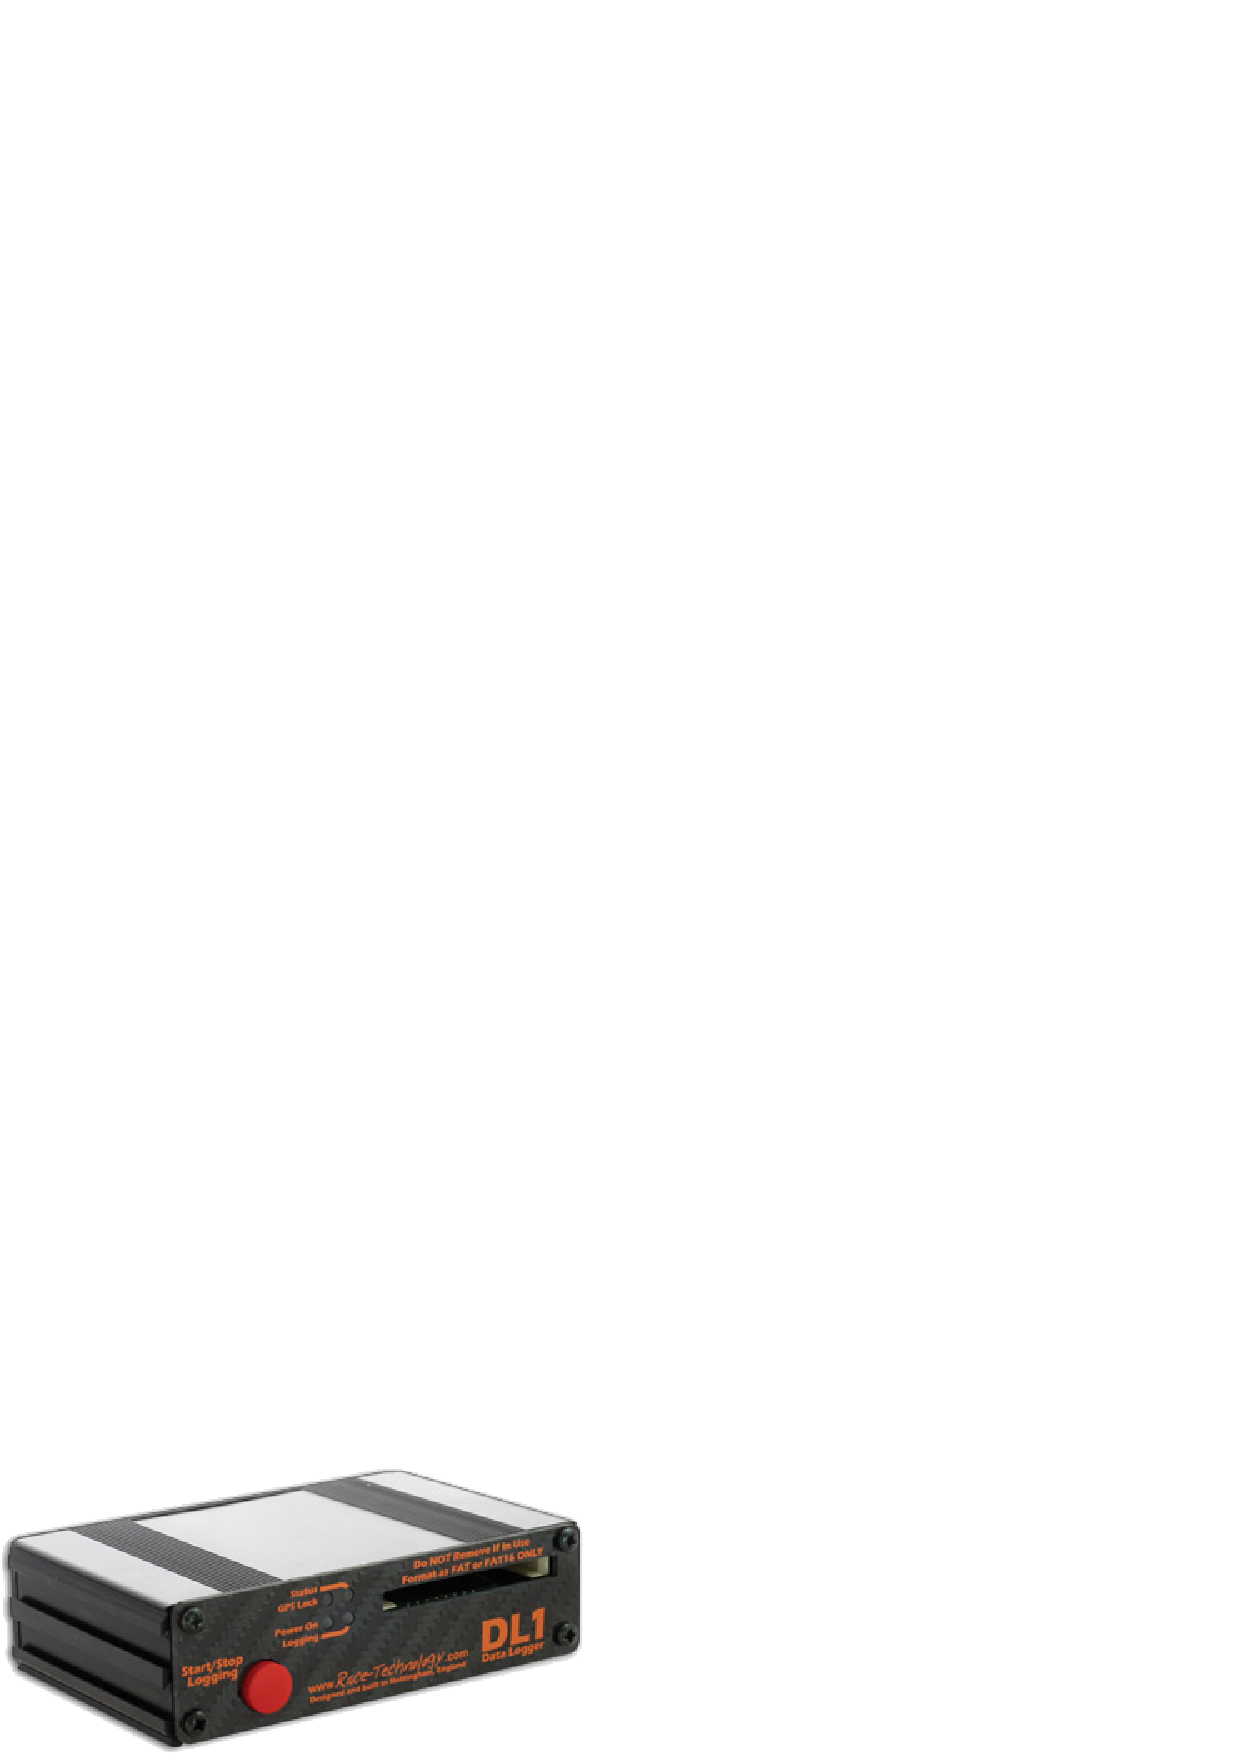
\includegraphics[scale=0.5]{Figures/dl1.png}
\caption{The Race Systems DL1 data acquisition device.}
\label{fig:dl1_product}
\end{figure}

\subsection{Previous Implementations and Shortcomings}

\subsubsection{Cellular Link}


\subsubsection{Off-the-Shelf XBee Link}

Both of these only worked with one device, weren't reliable, etc.



\section{Driver Interface}


\subsection{Overview}

Driver and crew needs easy access to data, easy control of on-board
systems


\subsection{Driver Controls}


\subsubsection{Transmission Control}

Upshift/Downshift

Activate other trans. control features, neutral find, etc., launch


\subsubsection{Engine Control}


\subsection{Vehicle Diagnostics}


\subsubsection{Critical Indicators}

Overheating, oil pressure, etc.


\subsubsection{Supplimentary Indicators}

information about telemetry, shift control, etc.


\subsection{Previous Implementations and Shortcomings}
